\section{Results}
\label{sec:results}

\subsection{Final Aggregate Comparison}

Table~\ref{tab:main-pragmatic} reports the complete best-tuned baseline comparison and ViPragSent-Final.  ViPragSent-Final reaches 84.3883 macro pragmatic F1, compared with 82.8250 for Vistral-7B, the strongest complete baseline.  The resulting aggregate difference is +1.5633 points.  Within the evaluated systems and this fixed evaluation, this is the highest recorded aggregate macro pragmatic F1.

\begin{table*}[t]
  \centering
  % Generated from answer/final_best_tuned/final_comparison.json.
\small
\setlength{\tabcolsep}{3pt}
\begin{tabular}{lccccccc}
\toprule
System & Implicit & Sarcasm & Irony & Idiom/fig. & Code-switch. & Mocking & Macro \\
\midrule
PhoBERT best-tuned & 60.85 & 77.37 & 96.32 & \textbf{97.30} & 78.99 & 79.45 & 81.71 \\
XLM-R-large best-tuned & 58.30 & 79.49 & 96.85 & \textbf{97.30} & 72.16 & 80.80 & 80.82 \\
Sailor-7B best-tuned & 57.43 & 78.57 & \textbf{97.41} & 97.15 & 81.28 & 81.31 & 82.19 \\
Vistral-7B best-tuned & 59.59 & 80.03 & 97.05 & 96.35 & \textbf{81.95} & 81.98 & 82.83 \\
\midrule
ViPragSent-Final & \textbf{67.98} & \textbf{80.28} & 97.02 & 97.18 & 81.82 & \textbf{82.05} & \textbf{84.39} \\
\bottomrule
\end{tabular}%

  \caption{Final pragmatic results (binary macro-F1 percentages). Bold indicates the best value in each column among the compared best-tuned baseline systems and ViPragSent-Final. The final system is a frozen, development-selected label-wise ensemble evaluated once on the canonical test set; the aggregate result does not imply per-label dominance.}
  \label{tab:main-pragmatic}
\end{table*}

\begin{figure}[t]
  \centering
  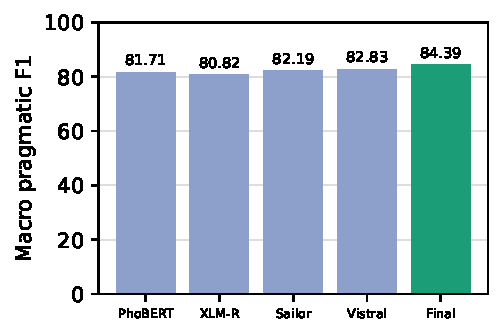
\includegraphics[width=\linewidth]{figures/final_macro_comparison}
  \caption{Macro pragmatic F1 for the complete best-tuned baseline systems and ViPragSent-Final. The comparison is an aggregate, equal-weight metric over six pragmatic labels.}
  \label{fig:final-macro}
\end{figure}

\subsection{Label-wise Comparison}

The aggregate comparison and the per-label-leader comparison answer different questions and are kept separate.  Relative to the strongest best-tuned baseline result for each label, ViPragSent-Final is ahead by 7.1359 points on implicit sentiment, 0.2463 on sarcasm, and 0.0726 on mocking.  It is below the label leader by 0.3955 points on irony, 0.1138 on idiom/figurative language, and 0.1294 on code-switching (Table~\ref{tab:final-gap}).

\begin{table*}[t]
  \centering
  \small
\setlength{\tabcolsep}{4pt}
\begin{tabular}{lccc}
\toprule
Comparison & Leader / score & ViPragSent-Final & Difference \\
\midrule
Aggregate macro F1 & Vistral-7B / 82.8250 & 84.3883 & +1.5633 \\
Implicit sentiment & PhoBERT / 60.8470 & 67.9829 & +7.1359 \\
Sarcasm & Vistral-7B / 80.0318 & 80.2781 & +0.2463 \\
Irony & Sailor-7B / 97.4132 & 97.0177 & -0.3955 \\
Idiom/figurative & PhoBERT/XLM-R-large / 97.2958 & 97.1820 & -0.1138 \\
Code-switching & Vistral-7B / 81.9458 & 81.8164 & -0.1294 \\
Mocking & Vistral-7B / 81.9802 & 82.0528 & +0.0726 \\
\bottomrule
\end{tabular}%

  \caption{Two comparison definitions. The first row compares aggregate system performance with Vistral-7B, the strongest complete baseline. The remaining rows compare each ViPragSent-Final label score with the strongest best-tuned baseline score for that label.}
  \label{tab:final-gap}
\end{table*}

\begin{figure}[t]
  \centering
  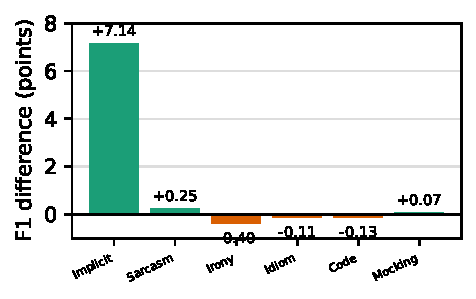
\includegraphics[width=\linewidth]{figures/final_label_gaps}
  \caption{Per-label difference between ViPragSent-Final and the strongest best-tuned baseline result for each label. The zero line distinguishes positive margins from localized deficits; the vertical scale is not truncated to exaggerate small differences.}
  \label{fig:final-gaps}
\end{figure}

\subsection{Uncertainty and Paired Comparisons}

The promoted bundle contains a post-hoc paired bootstrap over fixed test predictions for the final continuation versus its archived incumbent, using 1,000 replicates. The observed macro difference is +0.2979 points with a 95\% bootstrap interval of [-0.0714, 0.6463]; 94.4\% of replicates are positive. This interval is descriptive and was not used for selection. Comparable aligned prediction files for a paired final-versus-Vistral test and final-versus-each-label-leader tests are not present in the promoted bundle. We therefore report their point-estimate differences without a significance claim or invented interval, and do not apply Holm correction because no formal multi-hypothesis family is reported.

\subsection{Interpretation of Mixed Leadership}

The result is an aggregate-performance lead, not strict dominance of every pragmatic label.  All three localized deficits are below 0.40 points, while the implicit-sentiment gain is 7.1359 points and sarcasm and mocking also have positive margins.  Thus, the aggregate advantage is driven primarily by the large implicit-sentiment gain, supplemented by smaller gains on sarcasm and mocking.  These gains coexist with three localized deficits, producing the highest equal-weight macro pragmatic F1 among the evaluated complete systems.

\subsection{Development Progression and Legacy Analyses}

The progression from ViPragSent original (73.7469) through the previous optimized system (82.0699) and final incumbent (84.0904) to the promoted continuation (84.3883) is shown in Appendix~\ref{app:final-progression}.  These rows document development history and are not additional external baselines.

Existing ablation, source-stratified, low-resource, external-diagnostic, calibration, confusion, and annotation-agreement artifacts remain valid only for the system version named in each artifact.  In particular, the older 73.75 ablation behavior must not be attributed to ViPragSent-Final.

\subsection{Answer to the Research Questions}

ViPragSent-Final has the strongest aggregate macro pragmatic F1 among the evaluated systems, with a +1.5633-point margin over Vistral-7B.  This bounded aggregate result does not establish strict per-label superiority.
